\documentclass{article}
\usepackage{microtype}
\usepackage{graphicx}
\usepackage{booktabs}
\usepackage{hyperref}
\usepackage{tikz}
\usetikzlibrary{arrows.meta,positioning}

% Attempt to make text look nicer
\usepackage[accepted]{icml2025}
\usepackage{amsmath,amssymb,amsfonts}

\icmltitlerunning{Serving Is Learning: a Persistently Learning Device on Its Stream}

\begin{document}

\twocolumn[
\icmltitle{Serving Is Learning: Fusing Inference and Weight Updates \\
           in One Process on a Multiply-Free Substrate}
\icmlsetsymbol{equal}{*}
\begin{icmlauthorlist}
\icmlauthor{Anonymous}{anon}
\end{icmlauthorlist}
\icmlaffiliation{anon}{Anonymous Institution}
\icmlcorrespondingauthor{Anonymous}{anon@example.com}
\icmlkeywords{continual learning, predictive coding, tropical algebra, on-device learning, FPGA}
\vskip 0.3in
]

\printAffiliationsAndNotice{}

\begin{abstract}
Deployed models act and learn in different processes: an inference server
answers the stream while a separate training pipeline---with its own optimizer
workers, replay storage, activation memory, and synchronization---periodically
revises the weights. We ask whether that separation is necessary, and answer
by construction: on a tropical (max-plus) sequence model, where weights enter
additively and credit assignment reduces to routing errors through the
argmax/argmin caches the \emph{serving forward pass already produced}, a
single process can serve every token and, when a surprise gate fires, convert
the same forward pass into an exact training step. We measure the fused loop
at $1.38\times$ a forward pass in operation volume with gradients bitwise
equal to backpropagation's, machine-audited to contain zero multiplications.
In a pre-registered validation ladder we show the loop (i) captures
61--69\% of the frozen-to-oracle headroom on drifting streams; (ii) exposes a
law of surprise gating---any self-normalized $z$-gate is a fixed-quantile rate
limiter that cannot distinguish regimes---and its constructive fix, a
two-timescale absolute-margin gate that self-quiets by construction; (iii)
holds a Pareto frontier against a LoRA-periodic GPU incumbent tuned to win,
which needs $3.3\times$ our update compute and a $2.7\times$ activation-memory
class to match our quality; and (iv) sustains a 10M-token, five-era-cycle
\emph{life} in one process at $1.0063\times$ serving cost with weight-norm
equilibrium, bounded non-increasing interference, and a fully replayable
update stream carrying a sampled (5\%) zero-multiply audit. On real FPGA silicon the marginal power of learning-while-serving is
below the telemetry floor ($\le$1\,W on a $\sim$4\,W rail) while an A10G GPU
draws 79\,W of board power merely serving the same stream. Two pre-registered
negatives are reported with mechanisms. The individual components are largely
not new; the claim of this paper is the fused, audited, life-validated whole.
\end{abstract}

\section{Introduction}
\label{sec:intro}

Modern deployment separates \emph{acting} from \emph{learning}. Even systems
described as ``online'' learners---streaming RL agents, test-time-training
models, periodically fine-tuned services---maintain two computational
processes: a forward path that produces behavior, and a training path with its
own memory class (activation storage for backpropagation), its own workers,
and a synchronization discipline between the two. The separation is so
standard that it is rarely stated as an assumption.

This paper validates, end to end and on real silicon, a design in which the
separation is removed. The target property, fixed before any experiment and
used verbatim as the acceptance criterion, is:
\begin{quote}\itshape
a device sits on its stream; every example it serves, it may also learn from,
at about the cost of serving it twice, with no extra silicon, no extra memory
class, and no synchronization with anything else.
\end{quote}
We split this into two claims that prior work often conflates.
\textbf{Goal~A (mechanism):} one persistent process serves predictions
\emph{and} intermittently updates its own weights in place, at a small
measured multiple of serving cost. \textbf{Goal~B (retention):} what the
loop learns is retained usefully over the device's whole life---bounded
forgetting, weight-norm equilibrium, revisits that pay back. A system can
satisfy A while failing B; our ladder gates them separately.

\paragraph{Why a tropical substrate makes fusion possible.}
The enabling observation is algebraic. In a max-plus (tropical) network every
mixing operation is a maximum of sums, so each weight enters
\emph{additively} through the winning path. At hard routing the derivative of
any output with respect to any weight is an indicator of path membership:
credit assignment is exactly a gather--scatter--add over the argmax caches
that the forward pass computes anyway. Two consequences follow. First,
\emph{learning needs no multiplications}---we audit this mechanically, at
every gate of the ladder, on CPU and on FPGA. Second, \emph{learning needs no
second forward pass and no activation graph}: the serving forward's routing
caches are a sufficient statistic for an exact backward sweep. A cascaded
(one-sweep) predictive-coding update on this substrate equals the fully
settled iterative PC fixed point and equals backpropagation's gradient,
bitwise; we therefore make \emph{no claim of a better learning rule}. The
contribution is the schedule, the substrate, and the audit.

\paragraph{The single novel claim.}
Tropical and matmul-free architectures, predictive-coding/backprop
equivalences, surprise gating, and precision anchors all have prior or
contemporaneous art (\S\ref{sec:related}). What we believe is new is the
\textbf{fused, single-process serve-and-learn loop, built, measured, audited,
and validated over a device-scale life}---together with the negative results
that calibrate it. Concretely, we contribute:
\begin{enumerate}
\item \textbf{The fused loop (Goal A).} One forward serves the logits and
feeds the reverse sweep: measured $1.23\times$ wall / $1.38\times$ operation
volume versus serve-only, gradients bitwise-identical to backpropagation,
zero unwaived multiplications in the serve-and-sweep path
(\S\ref{sec:ladder}); optimizer arithmetic is a declared, recorded boundary.
\item \textbf{A law of surprise gating.} A $z$-scored gate normalized by its
own running statistics converges to firing at a fixed quantile of any
stationary distribution---it is a rate limiter, not a novelty detector, and
cannot self-quiet (measured at every threshold). A two-timescale
\emph{absolute-margin} gate self-quiets by construction and retains 90\% of
the benefit at a third of the updates (\S\ref{sec:gate}).
\item \textbf{An honest incumbent Pareto.} Against a LoRA-periodic dense
transformer tuned to win from an iso-quality warm start, the fused learner is
not dominated: matching its quality costs the incumbent $3.3\times$ the
update compute and a $2.7\times$ activation-memory class; the GPU keeps the
unconstrained-compute end (\S\ref{sec:pareto}).
\item \textbf{A device life (Goal B).} 10M served tokens over five rotated
domain cycles in one process: 60\% of frozen-to-oracle headroom captured at
$1.0063\times$ serving cost, firing collapsing from 1{,}275 to 45 kicks per
cycle, norm equilibrium, non-increasing interference, a sign-drift adversary
survived at $3.5\times$ its historical collapse horizon, and 0 violations in
1{,}236 audited kicks (\S\ref{sec:life}).
\item \textbf{Silicon.} The loop's components run bit-exactly on AWS F2
FPGAs; the marginal power of learning-while-serving is below the 1\,W
telemetry floor on a $\sim$4\,W rail, reported as the pre-registered floor
rather than a win, beside a measured 79\,W GPU board draw for serving the
same stream (\S\ref{sec:silicon}).
\item \textbf{Two mechanistic negatives.} Fisher merging of gated lives
fails (importance encodes \emph{when} a learner last fired, not what it
our substrate's pre-training quality in 1{,}150 steps vs.\ our 8{,}699
($\sim$70$\times$ less wall clock, cross-hardware; the ceiling is real). Both are part of
the record (\S\ref{sec:negatives}).
\end{enumerate}

All gates, pass/kill criteria, and demotion paths were pre-registered before
their runs. The Fisher negative fell inside a pre-registered informational
rider (its follow-up is now itself pre-registered); the capability ceiling
is reported as required context, not as a triggered branch.

\section{Related Work}
\label{sec:related}

\textbf{Tropical and multiplication-free networks.} The tropical-geometric
view of piecewise-linear networks is established
\citep{zhang2018tropical}, morphological/max-plus layers and state-space
variants are an active line \citep{morpmamba2024}, tropical attention has
contemporaneous treatment \citep{tropicalattention2025}, and
multiplication-free language models exist at billion scale
\citep{zhu2024matmulfree}. We use these substrates; we do not claim them.

\textbf{Predictive coding and its equivalences.} Predictive coding networks
\citep{rao1999predictive,millidge2022predictive} approximate or, under known
schedules, exactly reproduce backpropagation
\citep{whittington2017approximation,song2020can}. Our cascade update
instantiates the exact regime on a substrate where the sweep is
multiplication-free; the equivalence itself is the Z-IL lineage, not a new
theorem.

\textbf{Continual and online learning.} Elastic weight consolidation and its
Fisher-metric descendants \citep{kirkpatrick2017overcoming}, replay and
parameter-isolation methods, and the loss-of-plasticity results
\citep{dohare2024loss} frame Goal~B. Our anchor is EWC-shaped (precision from
the optimizer's own second moments); our contribution there is the negative
transfer result under sparse gated firing.

\textbf{Test-time and streaming adaptation.} Test-time training
\citep{sun2020test} and streaming deep RL \citep{elsayed2024streaming} adapt
online but retain the standard backpropagation memory class and, in RL
systems, a structural actor/learner split \citep{espeholt2018impala,
horgan2018distributed}; \S\ref{sec:agent} develops this contrast.

\textbf{Efficient fine-tuning.} LoRA \citep{hu2022lora} is the deployed
incumbent for periodic adaptation and is our tuned-to-win baseline.

\section{Substrate and Theory}
\label{sec:substrate}

\begin{figure}[t]
\centering
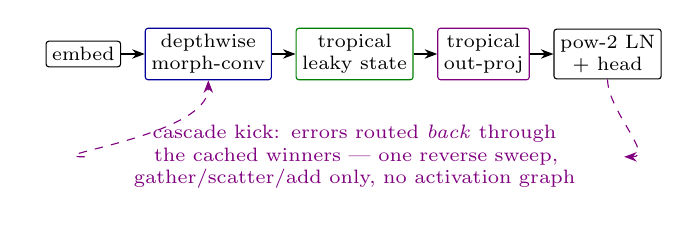
\begin{tikzpicture}[font=\scriptsize, node distance=3mm,
  box/.style={draw, rounded corners=1pt, inner sep=2.2pt, align=center},
  >={Stealth[length=1.6mm]}]
\node[box] (emb) {embed};
\node[box, right=of emb, draw=blue!60!black] (conv) {depthwise\\morph-conv};
\node[box, right=of conv, draw=green!50!black] (state) {tropical\\leaky state};
\node[box, right=of state, draw=violet] (proj) {tropical\\out-proj};
\node[box, right=of proj] (head) {pow-2 LN\\+ head};
\draw[->] (emb) -- (conv);
\draw[->] (conv) -- (state);
\draw[->] (state) -- (proj);
\draw[->] (proj) -- (head);
\node[below=4.5mm of state, text width=6.6cm, align=center]
  (cap) {\textcolor{violet}{cascade kick: errors routed \emph{back} through
  the cached winners --- one reverse sweep, gather/scatter/add only, no
  activation graph}};
\draw[->, violet, dashed] (head.south) to[out=-90,in=0] (cap.east);
\draw[->, violet, dashed] (cap.west) to[out=180,in=-90] (conv.south);
\end{tikzpicture}
\caption{The substrate (7 layers, $d{=}256$, BPE-1024). Every mixing op is
max/min-plus or a gather; the forward pass's argmax caches are the
credit-routing table for an exact, multiply-free backward sweep.}
\label{fig:arch}
\end{figure}

\paragraph{Model.} The learner is a MorphSSM language model
(Fig.~\ref{fig:arch}): token embeddings pass through $L{=}7$ layers of
depthwise morphological (max-plus) convolution, a tropical leaky state
$h_t=\max(u_t,\,h_{t-1}-\lambda)$ with learned non-negative leak (a
content-gated running maximum with bounded tropical spectral radius), and a
tropical dilation/erosion output projection; a power-of-two-scaled
normalization and a linear head produce logits. During training the hard
$\max$ is annealed from a soft relaxation ($\tau{:}\,0.5\!\to\!0$); all
results here operate the \emph{deployed} regime $\tau{=}0$.

\paragraph{Cascade $\equiv$ settled PC $\equiv$ BP.} Writing the network as a
feedforward DAG of tropical ops, a predictive-coding relaxation with the
standard chain-rule loss admits a closed-form fixed point; substituting it
layer by layer yields a single reverse sweep (the \emph{cascade}) whose
parameter updates equal the settled iterative PC updates and equal
backpropagation's gradients. We verify bitwise equality on every
architecture used here, including under asynchronous, partial-participation
sweeps. Because weights enter additively through winning paths, at
$\tau{=}0$ each gradient entry is a signed \emph{count-weighted sum of output
errors} routed through cached argmax indices: the sweep is
multiplication-free, and we enforce this with a dispatch-level auditor whose
waivers are declared: batch-mean divides, the LUT exponential, and---in the
research arm used for V2--V4---the AdamW/anchor update arithmetic, recorded
per step. The fully closed configuration (LUT loss + a shift-based
optimizer) audits clean end to end at V0; the reported lives ran the AdamW
arm.

\paragraph{The fused step.} \texttt{serve\_and\_learn} runs one forward pass,
returns the logits (the serving product), evaluates the gate on the window's
loss, and---only if fired---runs the reverse sweep \emph{on the caches that
forward already produced}, then steps the optimizer in place. There is no
second forward, no retained activation graph, no other process. Measured
against serve-only: $1.23\times$ wall clock, $1.38\times$ operation volume
(the pre-fusion harness paid $2.23\times$ wall / $2.38\times$ ops). Peak learning memory is
serve-class; the same cascade trained a $d{=}832$ variant where reverse-mode
autograd exhausted 44\,GB.

\section{The Gate: a Law and Its Fix}
\label{sec:gate}

\begin{figure}[t]
\centering
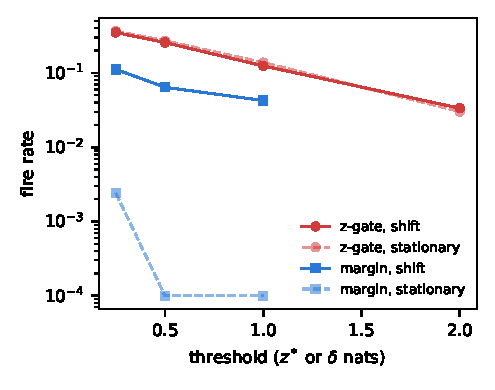
\includegraphics[width=0.86\columnwidth]{figs/fig_gatelaw.pdf}
\caption{The gate law. A $z$-scored gate (red) fires at a fixed quantile
regardless of regime---stationary and shifted streams are indistinguishable
at every threshold---because self-normalization erases regime information.
The two-timescale absolute-margin gate (blue) separates the regimes by
construction: it self-quiets on stationary data (dashed,
$2{\times}10^{-3}$ to $10^{-4}$) while storming at shifts.}
\label{fig:gatelaw}
\end{figure}

Always-on learning requires a decision rule for \emph{when} to convert a
serve into an update; we find the choice is not a tuning detail.
A gate that fires when the window loss exceeds its own running mean by
$z^\ast$ running standard deviations converges, on any stationary stream, to
firing at the fixed tail quantile $P(z>z^\ast)$: the boundary storms it
produces at distribution shifts are real (mean-lag), but its steady state is
regime-independent (Fig.~\ref{fig:gatelaw}). Empirically the fire rate on
stationary and hard-shift streams matched within 1.5 points at every
threshold. Such a gate can never satisfy the natural calibration criterion
(``quiet when there is nothing to learn'')---a property we believe deployed
surprise gates should be tested against.

The constructive fix removes the normalization: fire when a fast EMA of the
loss exceeds a slow EMA by an absolute margin $\delta$ (nats). On stationary
data both timescales converge and the gap vanishes; a shift opens the gap by
the loss jump itself. Measured: stationary fire rate $0.01$--$0.24\%$
versus the $z$-family's $27$--$36\%$ at the thresholds that preserve the
benefit ($z^\ast\le0.5$); raising $z^\ast$ to $1.0/2.0$ cuts stationary
firing to $13.8\%/3.0\%$ only by surrendering the shift benefit in lockstep
(headroom captured $0.55/0.25$) --- the rate is regime-independent at every
threshold. The margin gate retains 90\% of the benefit at $\delta{=}0.25$. Its known blind spot---entries into
intrinsically easier domains do not raise the loss---is handled at the
schedule level here and motivates difficulty-normalized surprise as future
work (\S\ref{sec:future}).

\section{Pre-Registered Validation Ladder}
\label{sec:ladder}

\begin{table}[t]
\caption{The ladder. Every gate pre-registered pass/kill criteria before its
run. HC = headroom captured $=1-R_{\mathrm{oracle}}/R^{\mathrm{frozen}}_{\mathrm{oracle}}$.}
\label{tab:ladder}
\vskip 0.05in
\centering
\scriptsize
\begin{tabular}{@{}lp{5.35cm}@{}}
\toprule
gate & verdict \\
\midrule
V0 & \textbf{pass}: fused loop $1.23\times$ wall / $1.38\times$ ops; grads
bitwise $\equiv$ BP; zero-multiply audit clean \\
V1 & \textbf{pass}: streams admissible (3.6--6.4 bits/tok regime headroom;
per-domain 6.7--10; wiki control 0.08); tokenizer identity exact \\
V2 & \textbf{pass}: regret $-1.6$ to $-3.0$ nats/tok vs.\ frozen; HC
0.61--0.69; $1.13\times$ serve (3 seeds) \\
V2b & \textbf{law}: $z$-gates cannot self-quiet (fixed-quantile); margin gate
replaces them \\
V3 & \textbf{pass}: frontier held vs.\ tuned LoRA-periodic (Fig.~\ref{fig:pareto}) \\
V4 & \textbf{pass}: the 10M-token life (Figs.~\ref{fig:life},\ref{fig:retention});
all Goal-B criteria \\
V4b & \textbf{negative}: Fisher merge loses to naive averaging under sparse
gated firing \\
V5 & \textbf{floor}: learning adds $\le$1\,W to a $\sim$4\,W rail on F2
(unresolvable); GPU serves the same stream at 79\,W board \\
\bottomrule
\end{tabular}
\vskip -0.1in
\end{table}

Streams are four text domains of 0.8--5\,MB (encyclopedic text,
Shakespeare, this repository's documentation, and its source code)
tokenized at BPE-1024; the learner is
warm-started from a text8-trained checkpoint (val 2.027 bits/byte), and all
adaptation runs at $\tau{=}0$. Prequential protocol throughout: every window
is scored by $\theta(t{-}1)$ \emph{before} any learning; a frozen twin is
scored on identical windows; per-domain oracles (converged specialists) give
the headroom denominator. Table~\ref{tab:ladder} summarizes.

\subsection{Does live learning pay? (V2)}
Across hard-shift, drift, and novel-vocabulary regimes the gated learner's
prequential regret versus its frozen twin was $-2.97$, $-2.92$, and $-1.58$
nats/token (3 seeds, s.d.\ $\le 0.023$), capturing 61--69\% of the
frozen-to-oracle headroom at $1.13\times$ amortized serving cost. On the
stationary control, firing (under the then-current $z$-gate) bought nothing:
the apparent $+0.10$ regret decomposed, once the margin gate silenced
updates, into a dropout-mode serving artifact (the no-update floor itself measures $+0.11$)---an accounting trap we flag
for prequential comparisons generally.

\subsection{The incumbent Pareto (V3)}
\label{sec:pareto}
\begin{figure}[t]
\centering
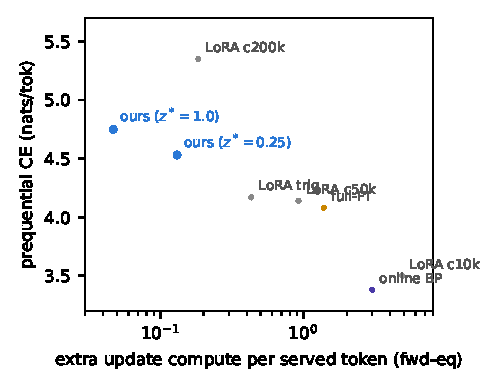
\includegraphics[width=0.9\columnwidth]{figs/fig_pareto.pdf}
\caption{Quality vs.\ update compute on identical streams. No incumbent cell
is below-and-left of ours; the cheapest cell beating our quality (LoRA,
drift-triggered) pays $3.3\times$ our update budget and a $2.7\times$
activation-memory class. GPUs keep the unconstrained-compute end.}
\label{fig:pareto}
\end{figure}
The incumbent is what deployment actually does: buffer the stream and
periodically run $K$ AdamW steps on LoRA adapters (rank $\times$ cadence
$\times$ lr swept; drift-triggered cadence included; full fine-tuning and
per-window online BP as anchors), from a dense transformer warm-started to
\emph{exactly} our checkpoint's pre-training quality (two-sided tolerance)
and served in eval mode so no artifact favors us. Fig.~\ref{fig:pareto}
shows the frontier. Two symmetric honest notes: the dense model reached that
warm-start quality in 1{,}150 steps versus our substrate's 8{,}699 (the
capability ceiling is real), and the incumbent's per-window online-BP arm \emph{hurts on
stationary data} ($+0.17$ regret)---unconditional always-on updating damages
any substrate; gating is a universal requirement, not a tropical patch.

\subsection{The life (V4)}
\label{sec:life}
\begin{figure}[t]
\centering
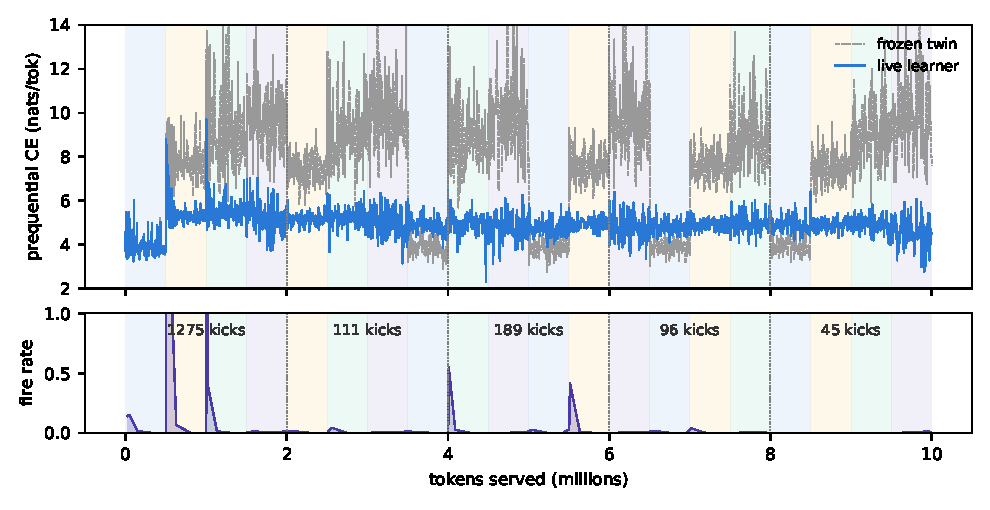
\includegraphics[width=\columnwidth]{figs/fig_life.pdf}
\caption{One process, 10M tokens, five rotated domain cycles. Top:
prequential CE of the live learner vs.\ its frozen twin. Bottom: gate fire
rate; kicks collapse $1{,}275\to45$ per cycle; two late eras are fully
silent and 42 of cycle 5's 45 kicks land in one storm at the final code
revisit---the device learned its world, then mostly just served.}
\label{fig:life}
\end{figure}
\begin{figure}[t]
\centering
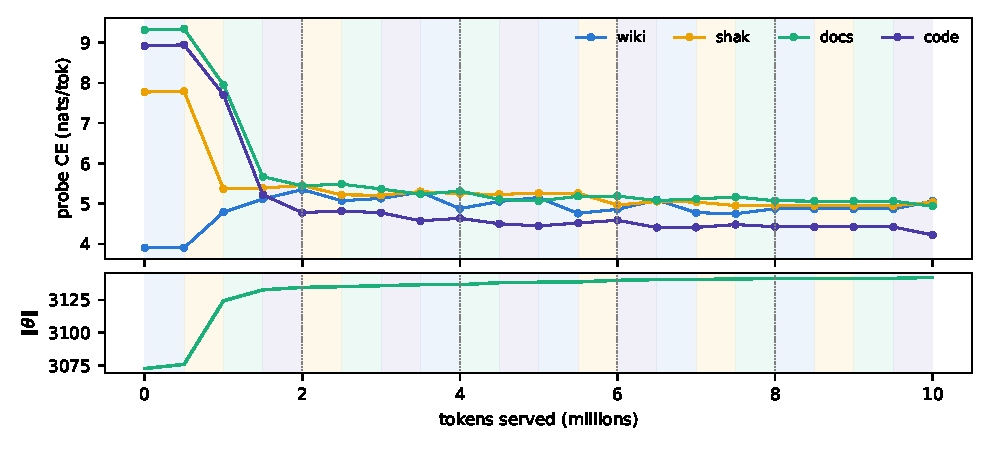
\includegraphics[width=\columnwidth]{figs/fig_retention.pdf}
\caption{Goal B. Top: held-out probe CE per domain at every era boundary;
after the first cycle the trade is stable and improves with revisits
(bounded, non-increasing interference). Bottom: weight norm reaches
equilibrium ($+2.3\%$ over the life; slope decelerates $12\times$).}
\label{fig:retention}
\end{figure}
The organism configuration (margin gate $\delta{=}0.25$, precision anchor
$\lambda{=}0.01$ on the optimizer's own second moments, learning-rate halving
on a fired-kick schedule) ran 104{,}160 windows in one process. Headroom
captured: $0.57{\pm}0.03$ over 3 seeds ($0.602/0.547/0.567$) at $1.006\times$ serving cost. Retention is a stability--%
plasticity \emph{trade}, reported as such: the wiki-specialist birth model
gave up $\sim$1.1 nats of its specialty for a generalist basin 2.7 nats
better on average, and held it with non-increasing interference across
cycles. A dedicated adversary rider ran 20{,}833 \emph{consecutive} updates
(gate bypassed) with the decay schedule---$3.5\times$ the horizon at which
our strict-optimizer runs historically collapsed---and ended better than
frozen (the adversary exercises the decay/anchor mechanism under the AdamW
research arm; the strict shift-optimizer variant, whose 6k-step collapse
set the horizon, remains untested at this horizon). A 5\% sampled dispatch audit covered 1{,}236 kicks across the four
lives: zero unwaived multiplications; the full update stream is replayable
from the seed and checkpoint chain.

\subsection{Fleet consolidation fails informatively (V4b)}
\label{sec:negatives}
Merging two disjoint-shard lives by Fisher-weighted averaging (each
learner's own Adam second moments as precision)---the recipe that had cut a
fleet-oracle gap by 97\% in a dense-update setting---\emph{loses to naive
averaging on every domain} here. Mechanism: under sparse gated firing the
second moments encode \emph{when} a rider last fired (fire rates differed
$4.0\%$ vs.\ $1.4\%$), not what it knows; and the riders converged to
overlapping generalist basins, so there were no true specialists to merge.
Importance for merging gated learners must be firing-normalized or
probe-based; we pre-register that follow-up rather than assume it.

\subsection{Silicon (V0 components, V5 energy)}
\label{sec:silicon}
The substrate's training kernels run on AWS F2 FPGAs with DSP multipliers
verifiably absent and known-answer tests bitwise-matching host goldens; a
trainer converged on-fabric during the measurement windows (CE
$4.15\to1.91$, trajectory equal to simulation). The energy question was
pre-registered with an honest-negative branch, which is what we report: on
the F2's core-rail telemetry (1\,W quantization) idle, serve, and
serve-and-learn measure 4.0--4.6\,W---\textbf{the marginal power of
learning is below the instrument's floor} ($\le$1\,W), and at the life's
1.65\% fire rate the amortized addition is unmeasurable. The trainer's
absolute figure is 5.3\,mJ per trained token-position (total rail, 756
tok/s, small kernel). The comparison that survives the rails-versus-board
caveat is regime-level: an A10G GPU drew a measured \textbf{79\,W of board
power merely serving} the same batch-1 stream at 26\% utilization
(5.6\,mJ/token; 16.0 under online BP). Board-level parity claims await
external instrumentation and are not made here.

\section{A Persistently Learning, Embodied Digital Agent}
\label{sec:agent}

The framing we find most consequential is not language modeling but agency.
Consider what ``online learning'' means in deployed RL systems. Actor--%
learner architectures \citep{espeholt2018impala,horgan2018distributed}
instantiate the acting policy and the learning process as \emph{different
programs}, often on different machines, coupled by replay buffers and
parameter servers; even single-process streaming RL
\citep{elsayed2024streaming} alternates environment steps with gradient
steps that traverse a distinct backward graph and memory class, and Dyna-style
agents \citep{sutton1991dyna} interleave acting with planning updates as
separate computations. In every case the agent \emph{stops being only an
actor} to learn: learning is a second activity scheduled against the first.

The loop validated here dissolves that boundary for the supervised-prediction
setting: \textbf{acting and learning share one computation}. The forward pass
that produces the agent's behavior (its next-token prediction) is,
unchanged, the sufficient statistic for its weight update; the gate decides
per-experience whether the act also becomes a lesson; the next act is taken
by the just-updated weights. There is no replay buffer, no learner replica,
no activation graph, no synchronization barrier---and the audit trail is a
property of the same stream. In the embodied-agent limit this is the
distinction between \emph{an agent that has a training pipeline} and
\emph{an agent whose experience is its training}: closer to the
always-plastic character of biological learning, where no organism schedules
a backward pass, than to the train/deploy dichotomy.

The V4 life gives this framing empirical content. The agent's whole
existence was acting on its stream; learning consumed 0.63\% additional
compute over that existence, concentrated exactly where its world changed
(1{,}275 kicks in the first cycle; 45 in the fifth), with its ``sleep-less''
plasticity bounded by the anchor rather than by a maintenance window. The
economics matter for embodiment: a device whose learning is energetically
invisible against its serving (\S\ref{sec:silicon}) can afford to be
\emph{always} plastic, whereas an agent that must run a second training
process on GPU-class hardware inherits that hardware's 79\,W floor and its
scheduling discipline. What this loop does \emph{not} yet provide is the RL
problem itself---credit over actions and delayed reward; here surprise is
the only teacher. Extending the fused loop from prediction to control,
without reintroducing the actor/learner split, is in our view the right next
problem (\S\ref{sec:future}).

\section{Discussion and Limitations}
\label{sec:discussion}

\textbf{What the evidence supports.} A single process can serve and learn at
$\approx1.4\times$ a forward pass per fired update and $\approx1.006\times$
amortized over a realistic life, exactly (bitwise) implementing gradient
descent, with no multiplications in the serve-and-learn sweep (optimizer
arithmetic declared) and no activation memory, on hardware where
the learning is energetically negligible. The claim is architectural and
systemic, not statistical: nothing here says this learner is more
sample-efficient than backpropagation---it \emph{is} backpropagation, on a
substrate and schedule that make it fusible into serving.

\textbf{Limitations.} (i) \emph{Capability ceiling}: at matched pre-training
quality a dense transformer trains in $7.6\times$ fewer steps
($\sim$70$\times$ less wall clock, cross-hardware) and its
frozen generalization is stronger; our substrate currently wins only the
always-on segment. (ii) \emph{Scale}: all results are at toy scale ($d{=}256$,
BPE-1024, $\sim$1.0M parameters); our larger silicon runs surfaced an unresolved
backward-path divergence that gates scaling. (iii) \emph{Board power}: the
FPGA rail measurement bounds core power only; full-card and ASIC numbers are
future instrumentation. (iv) \emph{Single seed} on the incumbent sweep
(the life is 3-seed: HC $0.57\pm0.03$, 0 audit violations across $3{\times}10^7$
served tokens). (v) The margin gate is blind to
easier-domain entries; difficulty normalization is unfinished.

\section{Future Work}
\label{sec:future}
Difficulty-normalized (excess-surprise) gating; firing-normalized importance
for fleet merging; closing the last non-audited optimizer arithmetic;
scaling through the localized backward divergence; and the agentic
extension: fusing action-conditional learning into the same single process,
so that an embodied agent's policy improvement---like its perception
here---is an occasional property of acting rather than a second life it
leads elsewhere.

\section*{Impact Statement}
This work targets low-power, auditable on-device learning. Positive impacts
include energy reduction and attributable (replayable) model updates in
regulated settings; risks include on-device adaptation drifting from
centrally validated behavior, which the audit-and-anchor machinery is
designed to bound. The four stream domains are public corpora (text8-derived encyclopedic
text, Shakespeare) and this project's own documentation and source code; no
other human data was used.

\bibliography{references}
\bibliographystyle{icml2025}

\end{document}
